\documentclass[12pt]{article}


% -------------------- PAQUETES --------------------
\usepackage[utf8]{inputenc}
\usepackage[spanish]{babel}
\usepackage[margin=2.54cm]{geometry}
\usepackage{graphicx}
\usepackage{xcolor}
\usepackage{enumitem}
\usepackage{parskip}
\usepackage{hyperref}
\usepackage{ulem} 
\usepackage{subcaption}


% -------------------- CARGA DE ARCHIVOS EXTERNOS --------------------
% ----------------- UTILIDADES PARA DAR UN MEJOR FORMATO DE DOCUMENTO -----------------  


\definecolor{azul}{rgb}{0.0039, 0.3098, 0.6196}


% Formato para el indice general ...........
\makeatletter
    \renewcommand{\@dotsep}{1.5}
    \renewcommand{\l@section}{\@dottedtocline{1}{1.5em}{2.3em}}
    \renewcommand{\l@subsection}{\@dottedtocline{2}{3.8em}{3.2em}}
    \renewcommand{\l@subsubsection}{\@dottedtocline{3}{7.0em}{4.1em}}
\makeatother

% --------- COMANDOS PERSONALIZADOS PARA LA PORTADA DE LAS TAREAS, TRABAJOS Y PROYECTOS ---------

\newcommand{\rutaLogo}[1]{\newcommand{\RutaLogo}{#1}}
\newcommand{\tema}[1]{\newcommand{\Tema}{#1}}
\newcommand{\etiquetaAutores}[1]{\newcommand{\EtiquetaAutores}{#1}}
\newcommand{\alumno}[1]{\newcommand{\Alumno}{#1}}
\newcommand{\materia}[1]{\newcommand{\Materia}{#1}}
\newcommand{\docente}[1]{\newcommand{\Docente}{#1}}
\newcommand{\ciclo}[1]{\newcommand{\Ciclo}{#1}}
\newcommand{\fecha}[1]{\newcommand{\Fecha}{#1}}
\newcommand{\periodo}[1]{\newcommand{\Periodo}{#1}}



% -------------------- DEFINICIÓN DE LA PORTADA --------------------
\rutaLogo{../../../../docs/img/logo-ista.png}
\tema{\\ \vspace{0.5cm} Guía Práctica N°2 - Datos Estructurados \\ \vspace{1.2cm}}
\etiquetaAutores{Integrantes:}
\alumno{Eduardo Mendieta\\Freddy Montalván\vspace{0.7cm}}
\materia{Introducción a Big Data \vspace{0.7cm}}
\docente{MSc. Ing. Carmen Tacuri Vintimilla \vspace{0.7cm}}
\ciclo{Primer Ciclo \vspace{0.7cm}}
\fecha{29 de julio de 2024 \vspace{0.7cm}}
\periodo{Abril 2024 - Agosto 2024}

\begin{document}

        \begin{titlepage}

    \centering

    \includegraphics[width=0.11\textwidth]{\RutaLogo} 

    \vspace{0.3cm}
    \textcolor{azul}{\Large \textbf{Instituto Superior Universitario Tecnológico del Azuay \\}}
    \vspace{0.3cm}
    \textcolor{azul}{\Large \textbf{Tecnología Superior en Big Data}}
    
    % 1. ---------------- TEMA -------------------------
    
    {\Large\textbf{\Tema}}
    
    % 2. ---------------- AUTOR(ES) -------------------------
    \textcolor{azul}{\large \textbf{\EtiquetaAutores} \\}
    \vspace{0.3cm}
    {\large \Alumno}

    % 3. ---------------- MATERIA -------------------------
    \textcolor{azul}{\large \textbf{Materia:} \\}
    \vspace{0.3cm}
    {\large \Materia}


    % 3. ---------------- DOCENTE -------------------------
    \textcolor{azul}{\large \textbf{Docente:} \\}
    \vspace{0.3cm}
    {\large \Docente}


    % 3. ---------------- Ciclo -------------------------
    \textcolor{azul}{\large \textbf{Ciclo:} \\}
    \vspace{0.3cm}
    {\large \Ciclo}


    % 3. ---------------- FECHA -------------------------
    \textcolor{azul}{\large \textbf{Fecha:} \\}
    \vspace{0.3cm}
    {\large \Fecha}

    % 3. ---------------- PERIODO -------------------------
    \textcolor{azul}{\large \textbf{Periodo Académico:} \\}
    \vspace{0.3cm}
    {\large \Periodo}
 
\end{titlepage}


        \tableofcontents
        \newpage

        \section*{\centering Guía Práctica N°2 - Datos Estructurados}

        % 1.Introducción: ...................................................
        \section{Introducción}
                En tecnologías de la información es fundamental crear modelos que permitan organizar y gestionar los datos. Estos modelos no solo facilitan la comunicación entre los técnicos y los usuarios finales, sino que también permiten realizar cambios de manera sencilla debido a su naturaleza simplificada. En esencia, un modelo de datos es una representación abstracta que organiza y documenta la información, actuando como puente entre el personal técnico y los demás empleados.

                El proceso de modelado de datos estructurados se divide en tres fases principales. La primera fase, el Diseño Conceptual, implica la identificación de las entidades clave del sistema y sus relaciones. Este paso define el alcance del problema que se desea resolver, utilizando elementos de modelado UML para representar las entidades de manera clara y comprensible.

                La siguiente fase, el Diseño Lógico, se centra en refinar estas entidades conceptuales en entidades lógicas más detalladas. En este punto, se definen las relaciones entre las entidades de manera más precisa, permitiendo una estructura más elaborada y coherente del modelo de datos. El uso de UML sigue siendo esencial para representar estas entidades y sus interacciones de forma detallada.

                Finalmente, el Diseño Físico transforma los diseños lógicos en estructuras físicas concretas, es decir, en tablas de bases de datos. Esta fase incluye la correlación de estas tablas con los espacios de almacenamiento y otros componentes de la base de datos, asegurando una implementación eficiente y funcional del modelo de datos.

                En el campo de la tecnología de la información, es vital tener la habilidad de analizar, modelar y proponer soluciones de modelado de datos estructurados, especialmente para su almacenamiento en bases de datos SQL. Esta práctica tiene como objetivo que los estudiantes se familiaricen con los diferentes modelos de datos estructurados, comprendiendo su importancia y aplicabilidad en el desarrollo de sistemas de información efectivos y bien organizados.
        
        % 2.Objetivos: ...................................................
        \newpage
        \section{Objetivos}
                \subsection{Objetivo general}
                        Generar los modelos conceptual, lógico y físico propuestos en la guía, de manera que comprendamos para qué sirve cada modelo y cómo se lleva a cabo su construcción.
                
                \subsection{Objetivos específicos}
                        \begin{itemize}
                                \item Utilizar cualquier software que nos permita modelar los ejemplos presentes en la guía.
                                \item Inferir sobre el uso y desarrollo de cada modelo.
                        \end{itemize}


        % 3.Paso a Paso: ...................................................
        \newpage
        \section{Paso a paso}
                \subsection{Modelamiento de la adopción de mascotas}
                        El modelo físico presentado está diseñado para gestionar un sistema de adopción de animales. Consta de tres tablas principales: \textit{Persona}, \textit{Adopcion} y \textit{Animal}. La tabla \textit{Persona} almacena información personal de los adoptantes, como su identificación, nombres, apellidos, fecha de nacimiento, dirección, móvil, email y estado de la persona. La tabla \textit{Animal} contiene datos sobre los animales disponibles para adopción, incluyendo el código del animal, nombre, color, edad, género, si es mestizo, carácter, especie, raza, tipo de edad, tamaño, fecha de rescate y estado del animal. 
                        
                        La tabla \textit{Adopcion} actúa como una tabla intermedia que relaciona a las personas con los animales adoptados, registrando la identificación de la persona y el código del animal, así como la fecha de adopción, si la adopción ha sido verificada y el estado de la adopción. Este modelo refleja una relación de \textit{muchos a muchos} entre las personas y los animales a través de la tabla de \textit{adopciones}, permitiendo un seguimiento detallado de las adopciones realizadas.
                        
                        \begin{figure}[!h]
                                \centering
                                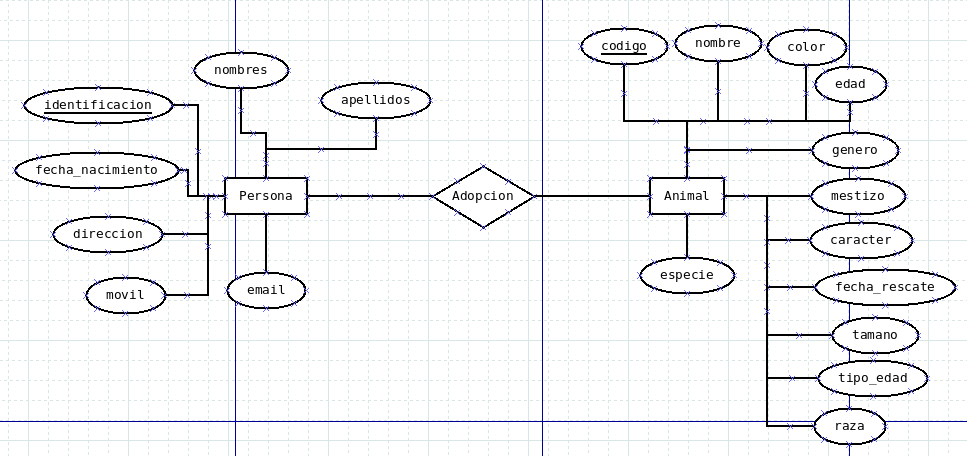
\includegraphics[width=0.85\textwidth]{img/ej1-1.png}
                                \caption{Modelo conceptual}
                        \end{figure}

                        \newpage
                        \begin{figure}[!h]
                                \centering
                                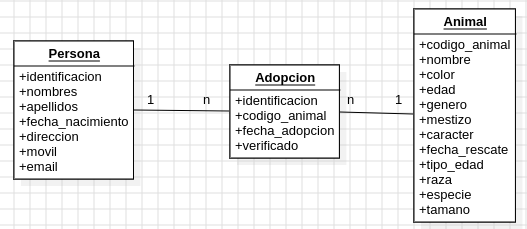
\includegraphics[width=0.85\textwidth]{img/ej1-2.png}
                                \caption{Modelo lógico}
                        \end{figure}

                        \begin{figure}[!h]
                                \centering
                                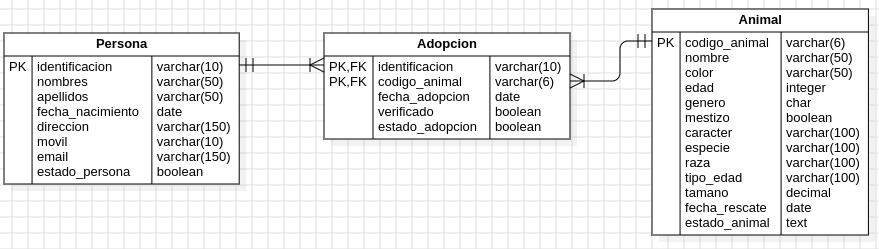
\includegraphics[width=0.9\textwidth]{img/ej1-3.png}
                                \caption{Modelo Físico}
                        \end{figure}
    
                
                
                \subsection{Modelamiento de compra de pasajes}
                        El modelo físico presentado está diseñado para gestionar un sistema de venta de pasajes de transporte. Consta de tres tablas principales: \textit{Cliente}, \textit{Compra} y \textit{Pasaje}. La tabla \textit{Cliente} almacena información personal de los clientes, como identificación, nombres, apellidos, fecha de nacimiento, dirección, móvil, email y estado del cliente. La tabla \textit{} contiene detalles sobre los pasajes disponibles, incluyendo el código del pasaje, línea de transporte, número de bus, destino, número de asiento, fecha de viaje, hora de salida, precio, andén terminal, tipo de bus, equipaje y estado del pasaje. 
                        
                        La tabla \textit{Compra} actúa como una tabla intermedia que relaciona a los clientes con los pasajes comprados, registrando la identificación del cliente y el código del pasaje, así como la fecha de compra, si se emitió un ticket en la terminal y el estado de la compra. Este modelo refleja una relación de \textit{muchos a muchos} entre los clientes y los pasajes a través de la tabla de \textit{compras}, permitiendo un seguimiento detallado de las transacciones realizadas.
                        
                        \newpage
                        \begin{figure}[!h]
                                \centering
                                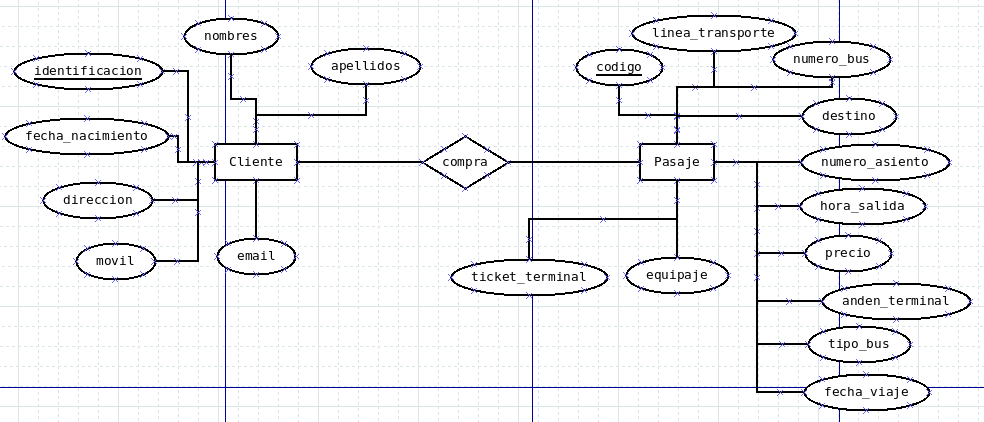
\includegraphics[width=0.85\textwidth]{img/ej2-1.png}
                                \caption{Modelo conceptual}
                        \end{figure}

                        \begin{figure}[!h]
                                \centering
                                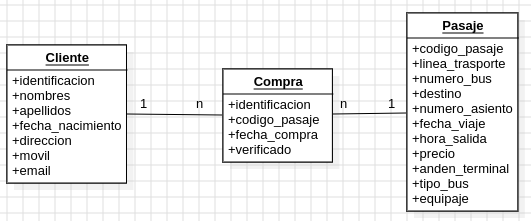
\includegraphics[width=0.85\textwidth]{img/ej2-2.png}
                                \caption{Modelo lógico}
                        \end{figure}

                        \begin{figure}[!h]
                                \centering
                                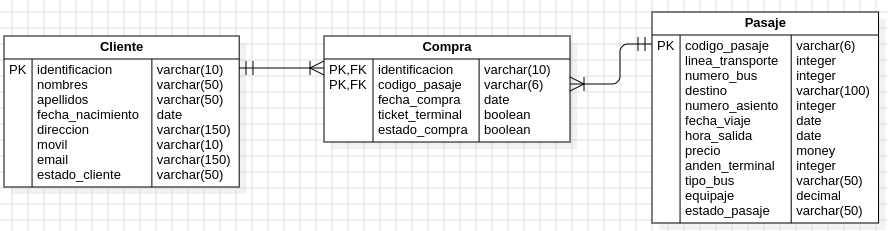
\includegraphics[width=1\textwidth]{img/ej2-3.png}
                                \caption{Modelo Físico}
                        \end{figure}
                        
                        
                \newpage
                \subsection{Modelamiento de venta de muebles}
                        El modelo físico de base de datos relacional presentado está diseñado para gestionar un sistema de ventas de muebles. Consta de tres tablas principales: \textit{Cliente}, \textit{Venta} y \textit{Mueble}. La tabla \textit{Cliente} almacena información personal de los clientes, como identificación, nombres, apellidos, fecha de nacimiento, dirección, móvil, email y estado del cliente. La tabla \textit{Mueble} contiene detalles sobre los muebles disponibles, incluyendo el código del mueble, tipo de mueble, si pertenece a una colección, color, número de piezas, tipo de material, modelo, variante, precio normal, precio en promoción y estado del mueble. 
                        
                        La tabla \textit{Venta} actúa como una tabla intermedia que relaciona a los clientes con los muebles comprados, registrando la identificación del cliente y el código del mueble, así como la fecha de venta, la factura y el estado de la venta. Este modelo refleja una relación de \textit{muchos a muchos} entre los clientes y los muebles a través de la tabla de ventas, permitiendo un seguimiento detallado de las transacciones realizadas.

                        \begin{figure}[!h]
                                \centering
                                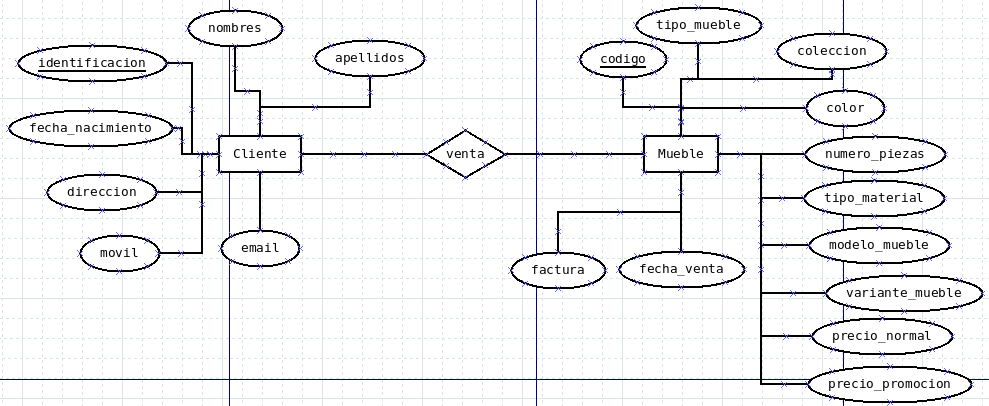
\includegraphics[width=0.85\textwidth]{img/ej3-1.png}
                                \caption{Modelo conceptual}
                        \end{figure}

                        \begin{figure}[!h]
                                \centering
                                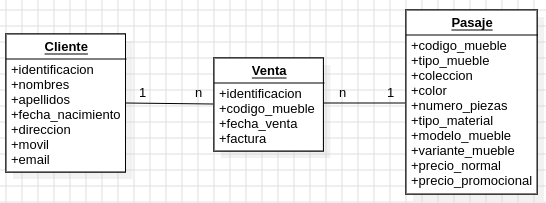
\includegraphics[width=0.85\textwidth]{img/ej3-2.png}
                                \caption{Modelo lógico}
                        \end{figure}

                        \newpage
                        \begin{figure}[!h]
                                \centering
                                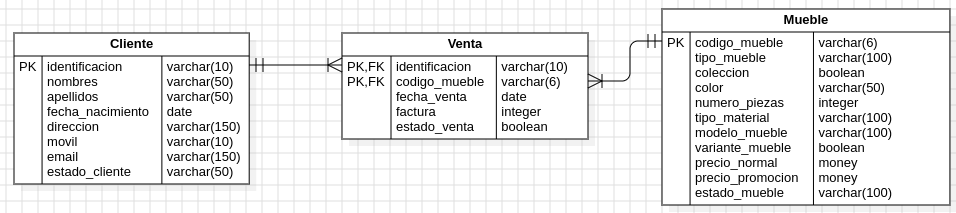
\includegraphics[width=1\textwidth]{img/ej3-3.png}
                                \caption{Modelo Físico}
                        \end{figure}



        % 4.Conclusiones: ...................................................
        \newpage
        \section{Conclusiones}
                \begin{enumerate}
                        \item La normalización de datos es crucial para evitar redundancias y garantizar la integridad de la base de datos. A través de la creación de tablas intermedias en los modelos \textit{Adopción, Compra y Venta}, se asegura que las relaciones de muchos a muchos se manejen adecuadamente, minimizando la duplicación de datos y facilitando un diseño más eficiente y manejable.
                        \item El diseño de una base de datos debe considerar el seguimiento detallado de las relaciones entre entidades. En cada uno de los modelos, se ha establecido una tabla intermedia que vincula dos entidades principales, permitiendo el registro y seguimiento de interacciones específicas , lo que ayuda a mantener una visión clara y organizada de las transacciones.
                        \item La estructura de una base de datos debe ser flexible y extensible para adaptarse a posibles cambios futuros. Al incluir atributos relevantes y detallar las características de cada entidad, los modelos permiten la adaptación a nuevas necesidades o cambios en los requisitos del sistema sin necesidad de una reestructuración completa.
                        \item La precisión en la definición de atributos es fundamental para asegurar la utilidad y la consistencia de la base de datos. La identificación de atributos específicos y relevantes en cada tabla permite que el sistema de base de datos soporte eficazmente las consultas y operaciones requeridas por los usuarios finales.
                        \item La relación entre clientes y entidades transaccionables se maneja eficientemente mediante tablas intermedias. Los modelos demuestran cómo utilizar tablas intermedias para gestionar relaciones complejas, lo que facilita la realización de un seguimiento exhaustivo de todas las interacciones comerciales, ya sea en el contexto de adopciones, compras de pasajes o ventas de muebles.
                \end{enumerate}


        % 5.Bibliografía: ...................................................
        \section{Bibliografía}
                \begin{itemize}
                        \item Guía practica proporcionada por la docente. 
                \end{itemize}


\end{document}